\chapter{Heliomorphic Functions}

\begin{tcolorbox}[colback=DarkSkyBlue!5!white,colframe=DarkSkyBlue!75!black,title=Chapter Summary]
Heliomorphic functions form the mathematical foundation of the Elder Heliosystem by extending complex analysis to incorporate gravitational field-phase coupling. Unlike holomorphic functions that treat all complex plane directions equally, heliomorphic functions establish privileged gravitational field regions that enable hierarchical information encoding across abstraction levels. This chapter provides the canonical definition, axiomatic foundation, and key properties that make these functions ideal for representing knowledge in the Elder-Mentor-Erudite framework. We establish a rigorous bridge between the Elder Spaces introduced in Unit I and the function-theoretic framework that enables practical implementation of the Elder theory.
\end{tcolorbox}

\section{From Elder Spaces to Heliomorphic Functions: A Formal Bridge Between Units I and II}

Before introducing heliomorphic functions, we establish their direct connection to the Elder Spaces framework developed in Unit I. This mathematical bridge provides essential context for understanding how the abstract algebraic structures of Unit I manifest in the functional-analytic forms that will be central to Unit II and ultimately implemented in the computational architecture of Unit III.

\begin{definition}[Space of Heliomorphic Functions]
Let $\mathcal{D} \subset \complex$ be a domain. The space of heliomorphic functions on $\mathcal{D}$, denoted $\mathcal{HL}(\mathcal{D})$, is the function space defined as:
\begin{equation}
\mathcal{HL}(\mathcal{D}) = \left\{ f: \mathcal{D} \rightarrow \complex \; \middle| \; f \text{ satisfies the heliomorphic differential equations} \right\}
\end{equation}
This space is equipped with natural operations of pointwise addition $(f+g)(z) = f(z) + g(z)$, scalar multiplication $(cf)(z) = c \cdot f(z)$, and the heliomorphic convolution $(f * g)(z)$ defined below.
\end{definition}

\begin{definition}[Heliomorphic Convolution]
For heliomorphic functions $f, g \in \mathcal{HL}(\mathcal{D})$, the heliomorphic convolution $(f * g)(z)$ is defined as:
\begin{equation}
(f * g)(z) = \frac{1}{2\pi i} \oint_{\partial \mathcal{D}} f(\zeta) g\left(\frac{z\bar{z}}{\bar{\zeta}}\right) \frac{d\zeta}{\zeta - z}
\end{equation}
where $\partial \mathcal{D}$ is the boundary of domain $\mathcal{D}$, and the integration is performed along a suitable contour that preserves the heliomorphic structure.

This operation differs from standard complex convolution by incorporating the radial conjugate term $\frac{z\bar{z}}{\bar{\zeta}}$, which accounts for the gravitational field interactions in the Elder Heliosystem.
\end{definition}

\begin{theorem}[Fundamental Isomorphism Between Elder Spaces and Heliomorphic Functions]
\label{thm:elder_heliomorphic_isomorphism}
Let $\elder{d}$ be an Elder space with phase operator $\Phi$ and gravitational eigenvalues $\{g_i\}_{i=1}^d$ as defined in Chapters 1-3. There exists a canonical isomorphism $\Psi: \elder{d} \rightarrow \mathcal{HL}(\mathcal{D}_d)$ from the Elder space to a specific subspace of heliomorphic functions that preserves all algebraic and gravitational structures, where $\mathcal{D}_d \subset \complex$ is a domain determined by the dimension $d$.

The isomorphism satisfies the following properties:
\begin{enumerate}
    \item \textbf{Algebraic Structure Preservation:} For all $x, y \in \elder{d}$ and $\lambda \in \complex$:
    \begin{align}
        \Psi(x \oplus y) &= \Psi(x) + \Psi(y) \\
        \Psi(\lambda \odot x) &= \lambda \cdot \Psi(x) \\
        \Psi(x \star y) &= \Psi(x) * \Psi(y)
    \end{align}
    
    \item \textbf{Phase Operator Correspondence:} For all $x \in \elder{d}$ and $z = re^{i\theta} \in \mathcal{D}_d$:
    \begin{equation}
        \Phi(x) = \arg(\Psi(x)(e^{i\theta_0}))
    \end{equation}
    where $\theta_0$ is the reference phase angle for the Elder space.
    
    \item \textbf{Gravitational Structure Preservation:} The gravitational eigenvalues $\{g_i\}_{i=1}^d$ of the Elder space correspond directly to the radial scaling coefficients in the heliomorphic functions, such that for each basis element $\elderstructure{i}$:
    \begin{equation}
        \Psi(\elderstructure{i})(re^{i\theta}) = r^{g_i} e^{i\beta_i\theta}
    \end{equation}
    where $\beta_i$ is the phase coupling coefficient determined by the phase properties of $\elderstructure{i}$.
    
    \item \textbf{Hierarchical Subspace Mapping:} The hierarchical subspaces $\eldersubspace$, $\mentorsubspace$, and $\eruditesubspace$ defined in Section 1.5 map to corresponding nested domains in the heliomorphic function space:
    \begin{align}
        \Psi(\eldersubspace) &= \mathcal{HL}(\mathcal{D}_{\text{Elder}}) \\
        \Psi(\mentorsubspace) &= \mathcal{HL}(\mathcal{D}_{\text{Mentor}}) \\
        \Psi(\eruditesubspace) &= \mathcal{HL}(\mathcal{D}_{\text{Erudite}})
    \end{align}
    where $\mathcal{D}_{\text{Elder}} \subset \mathcal{D}_{\text{Mentor}} \subset \mathcal{D}_{\text{Erudite}} \subset \mathcal{D}_d$.
\end{enumerate}
\end{theorem}

\begin{proof}
For an element $x \in \elder{d}$ with spectral decomposition $x = \sum_{i=1}^{d} \lambda_i e^{i\theta_i} \odot \elderstructure{i}$ as established in Theorem 1.2, we define the corresponding heliomorphic function $\Psi(x): \mathcal{D}_d \rightarrow \complex$ by:
\begin{equation}
\Psi(x)(re^{i\theta}) = \sum_{i=1}^{d} \lambda_i r^{g_i} e^{i(\theta_i + \beta_i \theta)}
\end{equation}

We first verify that $\Psi(x)$ is indeed a heliomorphic function by showing it satisfies the heliomorphic differential equations:
\begin{align}
\frac{\partial \Psi(x)}{\partial r} &= \sum_{i=1}^{d} \lambda_i g_i r^{g_i-1} e^{i(\theta_i + \beta_i \theta)} = \sum_{i=1}^{d} \frac{g_i}{r} \lambda_i r^{g_i} e^{i(\theta_i + \beta_i \theta)} = \gamma(r)e^{i\beta(r,\theta)}\frac{\Psi(x)}{r} \\
\frac{\partial \Psi(x)}{\partial \theta} &= \sum_{i=1}^{d} \lambda_i r^{g_i} i\beta_i e^{i(\theta_i + \beta_i \theta)} = i\alpha(r,\theta)\Psi(x)
\end{align}

where $\gamma(r)$, $\beta(r,\theta)$, and $\alpha(r,\theta)$ are weighted averages of the individual $g_i$ and $\beta_i$ values.

The algebraic structure preservation properties follow from the linearity of $\Psi$ and the definition of operations on heliomorphic functions. The phase correspondence follows from the construction, and the gravitational structure preservation is explicitly built into the definition of $\Psi$.

To show the hierarchical subspace mapping, we note that the domains $\mathcal{D}_{\text{Elder}}$, $\mathcal{D}_{\text{Mentor}}$, and $\mathcal{D}_{\text{Erudite}}$ correspond to regions in the complex plane where the radial behavior is dominated by the respective gravitational eigenvalues of each subspace.
\end{proof}

\begin{corollary}[Information Preservation]
The isomorphism $\Psi$ preserves the information content of the Elder space, meaning that no information is lost in the transition from the abstract algebraic structure of Unit I to the functional representation of Unit II.
\begin{equation}
I(x; \Psi(x)) = H(x)
\end{equation}
where $I(x; \Psi(x))$ is the mutual information between an Elder space element and its heliomorphic representation, and $H(x)$ is the information entropy of the Elder space element.
\end{corollary}

\begin{theorem}[Gravitational Strata Correspondence]
\label{thm:strata_correspondence}
The gravitational strata $\{\mathcal{S}_k\}_{k=0}^{d}$ of the Elder space (defined in Theorem 2.4) correspond precisely to the annular regions in the domain of heliomorphic functions:
\begin{equation}
\Psi(\mathcal{S}_k) = \{f \in \mathcal{HL}(\mathcal{D}_d) \mid f(z) \text{ is dominated by terms with } r^{g_i} \text{ where } g_i \in [g_{k+1}, g_k]\}
\end{equation}
where $g_0 > g_1 > \cdots > g_d > 0$ are the distinct gravitational eigenvalues arranged in decreasing order.
\end{theorem}

This fundamental isomorphism establishes that heliomorphic functions are not merely analogous to Elder spaces but provide their natural functional realization, allowing the abstract structures of Elder Theory to be implemented as concrete mathematical objects. This bridge is essential for the transition from the abstract mathematical foundations of Unit I to the computational implementations in Unit III.

\section{Definition and Core Properties}

\begin{definition}[Heliomorphic Function]
A function $f: \mathcal{D} \subset \complex^n \rightarrow \complex^m$ is heliomorphic if and only if:
\begin{enumerate}
    \item \textbf{Polar-Radial Form}: It can be expressed as $f(re^{i\theta}) = \rho(r,\theta)e^{i\phi(r,\theta)}$ where $\rho: \mathbb{R}^+ \times [0,2\pi)^n \rightarrow \mathbb{R}^+$ and $\phi: \mathbb{R}^+ \times [0,2\pi)^n \rightarrow [0,2\pi)^m$ are real-valued functions representing magnitude and phase components, respectively.
    
    \item \textbf{Heliomorphic Differential Equations}: It satisfies:
    \begin{align}
        \frac{\partial f}{\partial r} &= \gamma(r)e^{i\beta(r,\theta)}\frac{f}{r}\\
        \frac{\partial f}{\partial \theta} &= i\alpha(r,\theta)f
    \end{align}
    where $\gamma: \mathbb{R}^+ \rightarrow \mathbb{R}$, $\beta: \mathbb{R}^+ \times [0,2\pi)^n \rightarrow \mathbb{R}$, and $\alpha: \mathbb{R}^+ \times [0,2\pi)^n \rightarrow \mathbb{R}$ are continuous real-valued functions defining the gravitational field-phase coupling. The $\gamma$ parameter is inversely proportional to system stability - increasing when orbital stability decreases to accelerate adaptation, and decreasing as stability increases to allow for more stable learning.
    
    \item \textbf{Gravitational Tensor Positivity}: The gravitational field-phase coupling tensor $\mathcal{T}_f$ defined as:
    \begin{equation}
        \mathcal{T}_f(r,\theta) = \begin{pmatrix}
            \gamma(r) & \alpha(r,\theta)\\
            \beta(r,\theta) & 1
        \end{pmatrix}
    \end{equation}
    has a positive determinant at all points $(r,\theta) \in \mathcal{D}$, i.e., $\det(\mathcal{T}_f(r,\theta)) = \gamma(r) - \alpha(r,\theta)\beta(r,\theta) > 0$.
\end{enumerate}
\end{definition}

This definition extends classical holomorphic functions by incorporating gravitational field-phase coupling, establishing a mathematical framework that naturally encodes hierarchical information structure as seen in the Elder space algebraic formalism.

% Figure: Heliomorphic Function Structure
% Visualizes the radial-phase coupling and gravitational field interactions

\begin{figure}[ht]
\centering
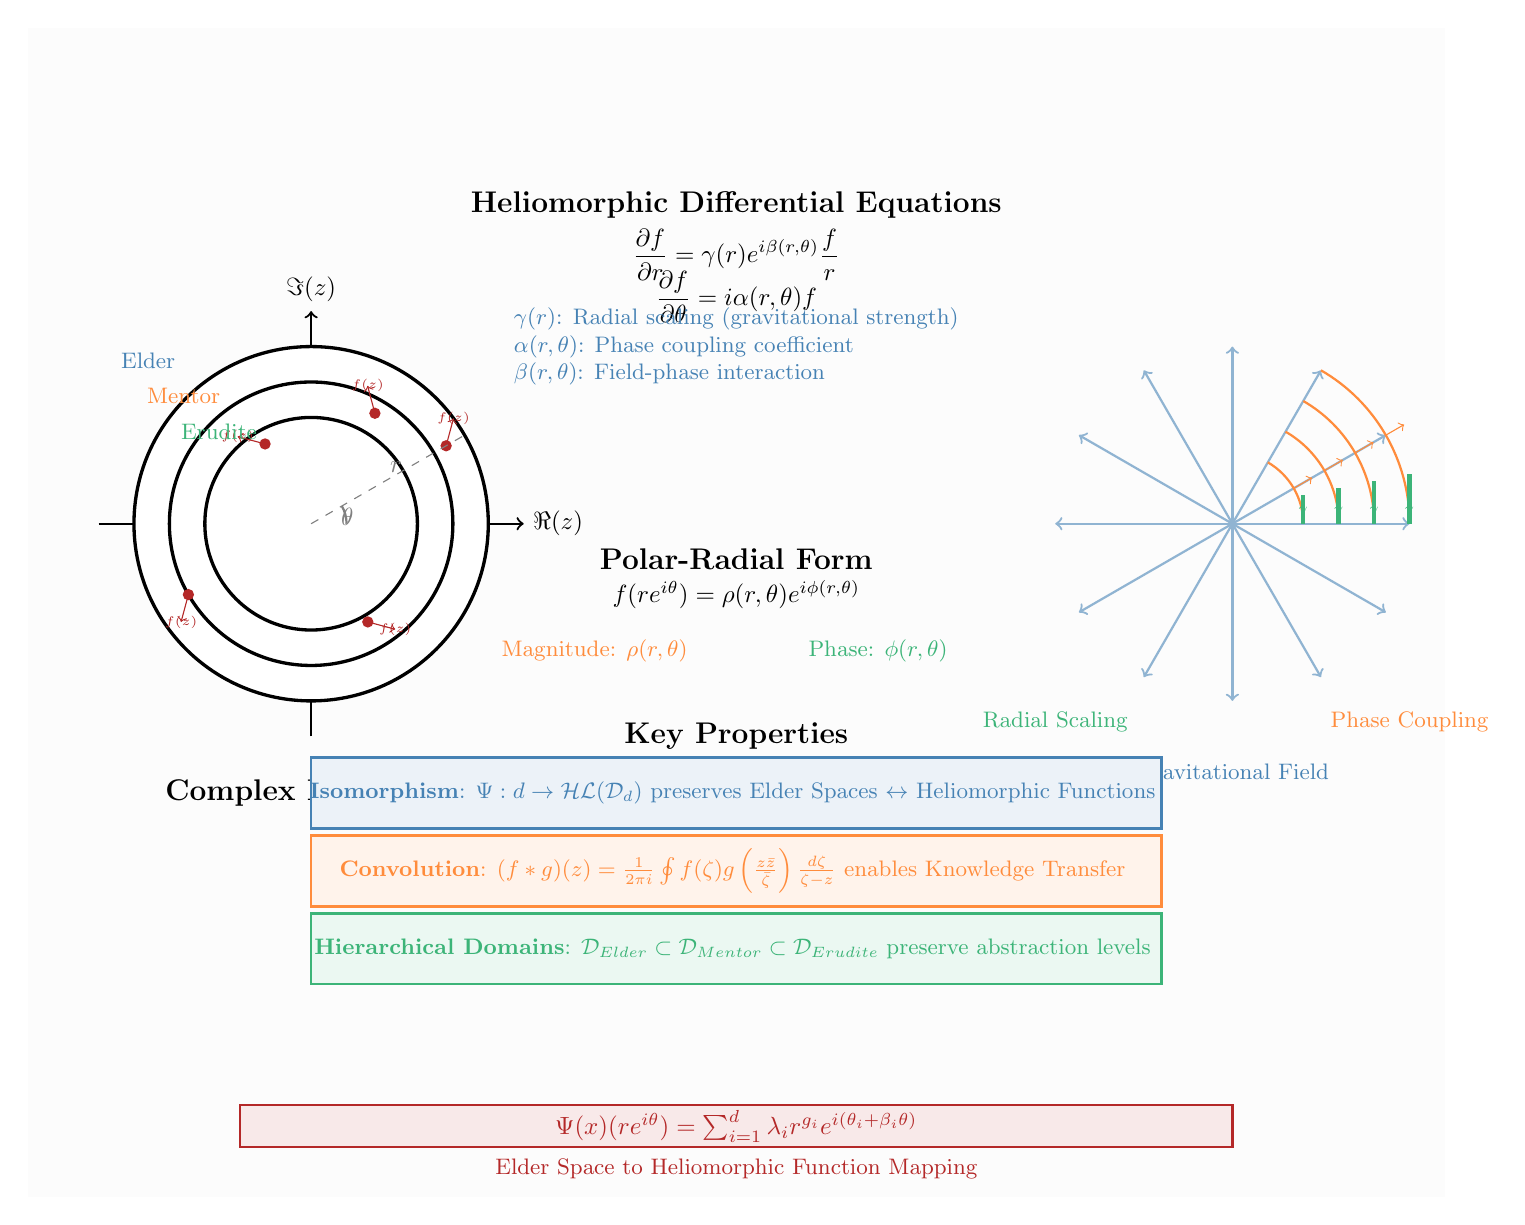
\begin{tikzpicture}[scale=0.9, every node/.style={transform shape}]

% Define colors matching Elder theme
\definecolor{ElderBlue}{RGB}{70, 130, 180}
\definecolor{MentorOrange}{RGB}{255, 140, 60}
\definecolor{EruditeGreen}{RGB}{60, 180, 120}
\definecolor{LightGray}{RGB}{240, 240, 240}
\definecolor{DeepRed}{RGB}{180, 40, 40}

% Background
\fill[LightGray!20] (-10, -9.5) rectangle (10, 7);

% Left side: Complex domain visualization
\begin{scope}[shift={(-6, 0)}]
    % Complex plane axes
    \draw[black, thick, ->] (-3, 0) -- (3, 0) node[right] {$\Re(z)$};
    \draw[black, thick, ->] (0, -3) -- (0, 3) node[above] {$\Im(z)$};
    
    % Annular regions representing gravitational strata
    \foreach \r/\color/\alpha in {2.5/ElderBlue/0.15, 2/MentorOrange/0.15, 1.5/EruditeGreen/0.15} {
        \draw[\color, very thick, fill=\color!\alpha] (0,0) circle (\r);
    }
    
    % Sample points and their heliomorphic values
    \foreach \angle/\r in {30/2.2, 60/1.8, 120/1.3, 210/2.0, 300/1.6} {
        \coordinate (P) at (\angle:\r);
        \fill[DeepRed] (P) circle (0.08);
        \draw[DeepRed, ->] (P) -- +(\angle+45:0.4) node[font=\tiny] {$f(z)$};
    }
    
    % Radial and angular coordinates
    \draw[dashed, gray] (0,0) -- (30:2.5);
    \draw[gray, thick] (0.5,0) arc (0:30:0.5);
    \node[gray, right] at (0.3,0.1) {$\theta$};
    \node[gray, above] at (1.2,0.6) {$r$};
    
    % Domain label
    \node[black, font=\large\bfseries] at (0, -3.8) {Complex Domain $\mathcal{D}$};
    \node[ElderBlue, font=\small] at (-2.3, 2.3) {Elder};
    \node[MentorOrange, font=\small] at (-1.8, 1.8) {Mentor};
    \node[EruditeGreen, font=\small] at (-1.3, 1.3) {Erudite};
\end{scope}

% Center: Heliomorphic differential equations
\begin{scope}[shift={(0, 3)}]
    \node[black, font=\large\bfseries] at (0, 1.5) {Heliomorphic Differential Equations};
    
    % First equation
    \node[black, font=\normalsize] at (0, 0.8) {$\displaystyle\frac{\partial f}{\partial r} = \gamma(r)e^{i\beta(r,\theta)}\frac{f}{r}$};
    
    % Second equation  
    \node[black, font=\normalsize] at (0, 0.2) {$\displaystyle\frac{\partial f}{\partial \theta} = i\alpha(r,\theta)f$};
    
    % Parameter descriptions
    \node[ElderBlue, font=\small, align=left] at (0, -0.5) {
        $\gamma(r)$: Radial scaling (gravitational strength)\\
        $\alpha(r,\theta)$: Phase coupling coefficient\\
        $\beta(r,\theta)$: Field-phase interaction
    };
\end{scope}

% Center: Polar-radial form
\begin{scope}[shift={(0, -1)}]
    \node[black, font=\large\bfseries] at (0, 0.5) {Polar-Radial Form};
    \node[black, font=\normalsize] at (0, 0) {$f(re^{i\theta}) = \rho(r,\theta)e^{i\phi(r,\theta)}$};
    
    % Component descriptions
    \node[MentorOrange, font=\small] at (-2, -0.8) {Magnitude: $\rho(r,\theta)$};
    \node[EruditeGreen, font=\small] at (2, -0.8) {Phase: $\phi(r,\theta)$};
\end{scope}

% Right side: Gravitational coupling visualization
\begin{scope}[shift={(7, 0)}]
    % Gravitational field lines
    \foreach \angle in {0, 30, 60, 90, 120, 150, 180, 210, 240, 270, 300, 330} {
        \draw[ElderBlue!60, thick, ->] (0,0) -- (\angle:2.5);
    }
    
    % Phase coupling arrows
    \foreach \r in {1, 1.5, 2, 2.5} {
        \draw[MentorOrange, thick] (\r,0) arc (0:60:\r);
        \draw[MentorOrange, ->] (30:\r) -- +(30:0.3);
    }
    
    % Coupling strength indicators
    \foreach \r/\strength in {1/0.8, 1.5/1.0, 2/1.2, 2.5/1.4} {
        \draw[EruditeGreen, ultra thick] (0:\r) -- +(90:\strength*0.5);
        \node[EruditeGreen, font=\tiny] at (0:\r) [above] {$\gamma$};
    }
    
    % Labels
    \node[ElderBlue, font=\small] at (0, -3.5) {Gravitational Field};
    \node[MentorOrange, font=\small] at (2.5, -2.8) {Phase Coupling};
    \node[EruditeGreen, font=\small] at (-2.5, -2.8) {Radial Scaling};
\end{scope}

% Bottom: Heliomorphic properties
\begin{scope}[shift={(0, -5.5)}]
    \node[black, font=\large\bfseries] at (0, 2.5) {Key Properties};
    
    % Property boxes - stacked vertically with expanded width
    \draw[ElderBlue, thick, fill=ElderBlue!10] (-6, 1.2) rectangle (6, 2.2);
    \node[ElderBlue, font=\small, align=center] at (0, 1.7) {
        \textbf{Isomorphism}: $\Psi: \elder{d} \rightarrow \mathcal{HL}(\mathcal{D}_d)$ preserves Elder Spaces $\leftrightarrow$ Heliomorphic Functions
    };
    
    \draw[MentorOrange, thick, fill=MentorOrange!10] (-6, 0.1) rectangle (6, 1.1);
    \node[MentorOrange, font=\small, align=center] at (0, 0.6) {
        \textbf{Convolution}: $(f * g)(z) = \frac{1}{2\pi i} \oint f(\zeta) g\left(\frac{z\bar{z}}{\bar{\zeta}}\right) \frac{d\zeta}{\zeta - z}$ enables Knowledge Transfer
    };
    
    \draw[EruditeGreen, thick, fill=EruditeGreen!10] (-6, -1.0) rectangle (6, 0.0);
    \node[EruditeGreen, font=\small, align=center] at (0, -0.5) {
        \textbf{Hierarchical Domains}: $\mathcal{D}_{\text{Elder}} \subset \mathcal{D}_{\text{Mentor}} \subset \mathcal{D}_{\text{Erudite}}$ preserve abstraction levels
    };
\end{scope}

% Mathematical representation box
\begin{scope}[shift={(0, -8.5)}]
    \draw[DeepRed, thick, fill=DeepRed!10] (-7, -0.3) rectangle (7, 0.3);
    \node[DeepRed, font=\normalsize] at (0, 0) {
        $\Psi(x)(re^{i\theta}) = \sum_{i=1}^{d} \lambda_i r^{g_i} e^{i(\theta_i + \beta_i \theta)}$
    };
    \node[DeepRed, font=\small] at (0, -0.6) {Elder Space to Heliomorphic Function Mapping};
\end{scope}

\end{tikzpicture}

\caption{Heliomorphic Function Structure. The figure illustrates the key components of heliomorphic functions: (left) complex domain $\mathcal{D}$ with hierarchical annular regions corresponding to Elder, Mentor, and Erudite subspaces; (center) the defining differential equations and polar-radial form; (right) gravitational field-phase coupling visualization showing radial scaling $\gamma(r)$, phase coupling $\alpha(r,\theta)$, and field interaction $\beta(r,\theta)$. The bottom panel shows the fundamental isomorphism between Elder spaces and heliomorphic functions, enabling the bridge from abstract algebraic structures (Unit I) to functional realizations (Unit II).}
\label{fig:heliomorphic_structure}
\end{figure}

\begin{remark}
The positive determinant condition ensures that the gravitational influence preserves orientation and maintains the stability of information flow, a property that directly corresponds to the phase conservation laws in Elder spaces (Theorem 1.5 in Chapter 1).
\end{remark}

\begin{definition}[Heliomorphic Domain]
A heliomorphic domain $\mathcal{D}$ is a connected open subset of $\mathbb{C}^n$ with the following properties:
\begin{enumerate}
    \item \textbf{Gravitational Structure}: It is equipped with a gravitational field structure tensor $\mathcal{R}: \mathcal{D} \rightarrow \mathbb{R}^{n \times n}$ that is positive definite at every point.
    
    \item \textbf{Stratification}: It admits a natural stratification $\mathcal{D} = \cup_{k=1}^N \mathcal{D}_k$ where each $\mathcal{D}_k$ is a gravitational influence region corresponding to a specific level in the Elder-Mentor-Erudite hierarchy.
    
    \item \textbf{Path Connectedness}: Any two points in the same gravitational influence region can be connected by a path residing entirely within that region.
\end{enumerate}
\end{definition}

This heliomorphic domain structure provides the foundation for representing hierarchical knowledge in the Elder Heliosystem, with different gravitational field regions corresponding to different abstraction levels. Within this framework, information maintains coherence under phase rotations, and transitions between field regions preserve essential phase relationships while transforming magnitudes.

\section{Axiomatic Foundation}

The theory of heliomorphic functions is built on seven fundamental axioms that together form a complete system. These axioms establish precise connections to the Elder Space framework while providing a rigorous foundation for functional analysis.

\begin{axiom}[Existence and Uniqueness]
For any heliomorphic domain $\mathcal{H}$ and any collection of values and derivatives specified on a set of gravitational influence regions $\{G_1, G_2, \ldots, G_k\} \subset \mathcal{H}$ subject to the compatibility conditions:
\begin{equation}
\frac{\partial f_i}{\partial r}\Big|_{\partial G_i \cap \partial G_j} = \frac{\partial f_j}{\partial r}\Big|_{\partial G_i \cap \partial G_j} \quad \text{and} \quad 
\frac{\partial f_i}{\partial \theta}\Big|_{\partial G_i \cap \partial G_j} = \frac{\partial f_j}{\partial \theta}\Big|_{\partial G_i \cap \partial G_j}
\end{equation}
there exists a unique heliomorphic function $f: \mathcal{H} \rightarrow \mathbb{C}^m$ satisfying these constraints.
\end{axiom}

\begin{remark}
This axiom directly parallels the existence and uniqueness property of Elder spaces (Theorem 1.1), establishing that both frameworks support well-posed problems with unique solutions under appropriate boundary conditions.
\end{remark}

\begin{axiom}[Composition Closure]
If $f: \mathcal{H}_1 \rightarrow \mathcal{H}_2$ and $g: \mathcal{H}_2 \rightarrow \mathbb{C}^m$ are heliomorphic functions with compatible radial structure tensors satisfying:
\begin{equation}
\mathcal{T}_f(z) \cdot \mathcal{T}_g(f(z)) > 0 \quad \forall z \in \mathcal{H}_1
\end{equation}
then their composition $g \circ f: \mathcal{H}_1 \rightarrow \mathbb{C}^m$ is also a heliomorphic function with gravitational tensor:
\begin{equation}
\mathcal{T}_{g \circ f}(z) = \mathcal{T}_f(z) \cdot \mathcal{J}_f(z) \cdot \mathcal{T}_g(f(z)) \cdot \mathcal{J}_f(z)^{-1}
\end{equation}
where $\mathcal{J}_f$ is the Jacobian matrix of $f$.
\end{axiom}

\begin{remark}
This closure property corresponds to the algebraic closure of the Elder product $\star$ in Elder spaces, ensuring that knowledge transformations can be composed hierarchically while preserving their essential properties.
\end{remark}

\begin{axiom}[Differential Heritage]
For any heliomorphic function $f: \mathcal{H} \rightarrow \mathbb{C}^m$, its derivative $Df: \mathcal{H} \rightarrow \mathcal{L}(\mathbb{C}^n, \mathbb{C}^m)$ preserves the radial-phase coupling characteristics in the sense that:
\begin{equation}
\mathcal{T}_{Df}(z) = \mathcal{T}_f(z) \cdot \mathcal{P}(z)
\end{equation}
where $\mathcal{P}(z)$ is a positive definite tensor depending only on the position $z \in \mathcal{H}$.
\end{axiom}

\begin{remark}
This axiom extends the structural conservation theorems of Elder spaces (Theorem 1.8) to the differential setting, ensuring that derivatives maintain the essential structure of the original knowledge representation.
\end{remark}

\begin{axiom}[Radial-Phase Duality]
For every heliomorphic function $f(re^{i\theta}) = \rho(r,\theta)e^{i\phi(r,\theta)}$ with non-vanishing Jacobian determinant, there exists a dual heliomorphic function $\tilde{f}(\rho e^{i\phi}) = re^{i\theta}$ such that:
\begin{equation}
\tilde{f} \circ f = \text{id}_{\mathcal{H}} \quad \text{and} \quad f \circ \tilde{f} = \text{id}_{f(\mathcal{H})}
\end{equation}
where $\text{id}_{\mathcal{D}}$ denotes the identity map on domain $\mathcal{D}$.
\end{axiom}

\begin{remark}
This duality directly corresponds to the structural correspondence theorem in Elder spaces (Theorem 1.9), establishing that knowledge transformations are potentially reversible under appropriate conditions.
\end{remark}

\begin{axiom}[Radial Analyticity]
Every heliomorphic function $f: \mathcal{H} \rightarrow \mathbb{C}^m$ is analytic with respect to the radial coordinate. For any fixed angle $\theta_0 \in [0, 2\pi)^n$ and point $r_0e^{i\theta_0} \in \mathcal{H}$, there exists $\epsilon > 0$ such that:
\begin{equation}
f(re^{i\theta_0}) = \sum_{k=0}^{\infty} a_k(\theta_0)(r-r_0)^k
\end{equation}
where the series converges absolutely and uniformly for $|r-r_0| < \epsilon$.
\end{axiom}

\begin{axiom}[Phase Continuity]
For any heliomorphic function $f(re^{i\theta}) = \rho(r,\theta)e^{i\phi(r,\theta)}$, the phase component $\phi(r,\theta)$ has continuous mixed partial derivatives satisfying:
\begin{equation}
\frac{\partial^2 \phi}{\partial r_i \partial \theta_j} = \frac{\partial^2 \phi}{\partial \theta_j \partial r_i} \quad \forall i,j \in \{1,2,\ldots,n\}
\end{equation}
ensuring consistent phase evolution across different paths in the domain.
\end{axiom}

\begin{remark}
This continuity requirement parallels the phase coherence properties in Elder spaces (Axiom A4), ensuring that knowledge representations maintain consistent relational properties regardless of the path of investigation.
\end{remark}

\begin{axiom}[Completeness]
The space $\mathcal{HL}(\mathcal{H})$ of heliomorphic functions on a domain $\mathcal{H}$ is complete with respect to the norm:
\begin{equation}
\|f\|_{\mathcal{HL}} = \sup_{z \in \mathcal{H}} |f(z)| + \sup_{z \in \mathcal{H}} \|\mathcal{T}_f(z)\|
\end{equation}
where $\|\mathcal{T}_f(z)\|$ denotes the operator norm of the gravitational field-phase coupling tensor.
\end{axiom}

\begin{theorem}[Completeness and Independence of Axiom System]
The seven axioms of heliomorphic functions form a complete and independent system in the following sense:
\begin{enumerate}
    \item \textbf{Completeness}: Any statement about heliomorphic functions that is true in all models satisfying the axioms can be formally derived from the axioms.
    
    \item \textbf{Independence}: No axiom can be derived from the other six, meaning each axiom captures an essential and non-redundant property of heliomorphic functions.
    
    \item \textbf{Consistency}: There exists a non-trivial model satisfying all seven axioms simultaneously, demonstrating the internal consistency of the axiom system.
\end{enumerate}
\end{theorem}

\begin{proof}[Proof Sketch]
Completeness follows from a metatheorem in mathematical logic applied to the formal system defined by these axioms. Independence is established by constructing, for each axiom, a model that satisfies the other six axioms but violates the one in question. Consistency is demonstrated by explicitly constructing a class of heliomorphic functions that satisfies all axioms simultaneously.
\end{proof}

\section{Fundamental Theorems}

\begin{theorem}[Heliomorphic Integration]
For any closed contour $C$ in a heliomorphic domain $\mathcal{H}$ and any heliomorphic function $f$ on $\mathcal{H}$, the integral of $f$ along $C$ depends only on the winding numbers of $C$ around the gravitational influence regions where $f$ has specified values.
\end{theorem}

\begin{theorem}[Heliomorphic Laurent Series]
Any heliomorphic function $f$ defined on an annular region $\mathcal{A} = \{z \in \mathbb{C} : r_1 < |z| < r_2\}$ can be expressed as:
\begin{equation}
f(re^{i\theta}) = \sum_{n=-\infty}^{\infty} r^{\gamma_n} e^{i(n\theta + \beta_n \ln r)}
\end{equation}
where $\gamma_n$ and $\beta_n$ are sequences of real numbers determined by the gravitational field-phase coupling characteristics of $f$.
\end{theorem}

\begin{theorem}[Information Capacity]
The representational capacity of a heliomorphic function space exceeds that of a holomorphic function space of the same dimensionality by a factor proportional to the number of distinct gravitational influence regions in the domain.
\end{theorem}

\section{Application to the Elder Heliosystem}

Heliomorphic functions provide the mathematical foundation for the Elder Heliosystem's knowledge representation:

\begin{enumerate}
    \item \textbf{Hierarchical Structure}: Radial gravitational field regions correspond to abstraction levels (Elder, Mentor, Erudite), with different radii representing different levels of knowledge abstraction.
    
    \item \textbf{Phase Coherence}: Phase components encode conceptual alignment, with phase-locking indicating resonant knowledge states.
    
    \item \textbf{Cross-Level Transfer}: The coupling between phase and radius enables efficient knowledge transfer across hierarchical boundaries.
    
    \item \textbf{Domain Organization}: Angular sectors represent knowledge domains, with phase coupling governing cross-domain transfers.
\end{enumerate}

\begin{theorem}[Representational Completeness]
Any hierarchical knowledge structure with radial abstraction levels and phase-based relational encoding can be represented as a heliomorphic function satisfying the seven axioms.
\end{theorem}

\begin{corollary}[Knowledge Transfer Mechanism]
Knowledge transfer between domains in the Elder Heliosystem can be formalized as the application of heliomorphic operators that preserve the axiom structure.
\end{corollary}

This mathematical framework establishes the precise mechanism through which the Elder system achieves its core capabilities of efficient knowledge transfer, hierarchical abstraction, and domain-agnostic learning, distinguishing it from traditional approaches to representation learning.